\chapter{Zone Control}
\label{sec:zoneControl}

After occupancy assessment, the next stage of Smart Zoning is hardware control,
or {\em zone control}. This involves deciding on and actuating the HVAC system
with appropriate parameters and opening, or closing, the appropriate dampers in
order to direct conditioned air through the house. In this section we describe
the goals of zone control, the challenges that have to be overcome in
implementing it, and our approach to implementing this part of Smart Zoning. 

\section{Goals}
\label{sec:zoneControlGoals}

%% - Condition only when used
%%  - ``Occ'' -> ``On''
%%  - ``Unocc'' -> ``Off''

Since Smart Zoning attempts to minimize the energy wasted in conditioning unused
rooms, the goal of zoning control is to only condition rooms when they are
used. In the ideal case this can be achieved by turning on the equipment
conditioning a room when the room is occupied and turning it off when the room
becomes unoccupied. Yet, this is complicated when implementing room-level zones
using a centralized HVAC system. 

%% - But, zones are not independent

The first complication arises due to the thermal dependence between
rooms. Houses are not designed with rooms being thermally isolated because it is
conditioned by a single piece of equipment and the flow of air from all the
rooms towards a thermostat and return vent is desired. Thus, when attempting to
zone a house at the room level, it is necessary to take into consideration the
thermal interaction between dynamically generated zones.
 
%% - Single piece of equipment

Using a single piece of equipment, instead of heating and cooling units that can
be manipulated for each room individually, such as window air-conditioning
units, complicates zoning control because the fine-grained equipment control
that is necessary for room-level zoning cannot be easily achieved. A room-level
unit cannot be turned on or off as a resident enters or leaves a room and the
effect, across multiple rooms, of actuating the HVAC system has to be taken into
consideration. 

%% - How to control equipment based on multiple conflicting zone states

Finally, a zone control algorithm has to make decisions on equipment actuation
based on multiple conflicting zone states. For instance, a particular occupied room could
be too hot or too cold while another occupied room has to be conditioned, or one
room may require stage 2 conditioning, due to it being further away from the
setpoint than another room that requires stage 1 conditioning. The zone control
algorithm has to decide between these conflicting requirements while attempting
to minimize energy consumption without compromising occupant comfort. Due to the
above constraints of room-level zoning using a single piece of equipment, a
sophisticated zone controller is necessary to achieve the goal of conditioning
rooms only when used. 

\section{Challenges}
As we briefly pointed out above, zone control for room-level zoning using a
centralized HVAC system is challenging. In this section we present some of the
challenges that have to be overcome in implementing the zone controller for
Smart Zoning. 

%% - Interdependence between zones

\subsection{Interdependence Between Zones}

The first challenge is the interdependence between zones which is caused by all
the rooms sharing the same network of HVAC ducts. Thus, opening and closing
certain ducts, using dampers, has an effect on the airflow through other
ducts. For instance, if two rooms are services by branching ducts off a common
trunk duct, closing off one of the rooms would increase the airflow rate into
the other room. Thus, knowing the effect of closing various combinations of
dampers is essential in deciding on dynamic zones. A simple solution would be to
know the layout of ducts in the house being retrofitted, but this may not always
be known by the homeowners. Therefore, we present a method based on airflow
measurements from the registers which can be easily taken using a handheld
airflow meter.

%% - Minimum airflow

\subsection{Minimum Airflow}
\label{sec:minAirflow}

As described in Section~\ref{sec:zoneControlGoals}, the centralized HVAC system
poses a challenge to room-level zoning and one of the major reasons for this is
the minimum airflow requirement for forced-air HVAC systems. These systems rely
on forcing air over a condensation coil, transferring heat between the
refrigerant and the air, and them delivering the air through a series of ducts
to the rooms of a house. Ducts are usually properly sized so that most of the
air delivered by the fan exits the ducts, which prevents pressure buildup within
the ducts, and enables a constant flow of air over the coil. Ducts are also
sized to distribute air to rooms depending on the size of the room, with larger
rooms having more registers and wider ducts than smaller rooms. 

Room-level zoning requires these ducts to be closed which decreases the amount
of air that can leave the ducts through the registers. This causes leakage
through openings such as insufficiently insulated joints and could even cause
pressure buildup within the ducts that slows down the flow of air over the
coil. This {\em back-pressure} could damage the compressor due to insufficient
thermal flow between the refrigerant and air causing the refrigerant to not
fully vaporize before flowing back into the compressor. Thus, ensuring a minimum
airflow out of the registers when deciding on which dampers to close is a
challenge that has to be overcome to ensure equipment safety.

%% - Efficiency dependence
%%   - 2 rooms open > 1 room open
%%   - If smaller than load, BAD

\subsection{Efficiency Dependence}
\label{sec:efficiencyDependence}

%------------------------------------------------------------------------------
% Figure 5
\begin{figure}[t]
\centering{
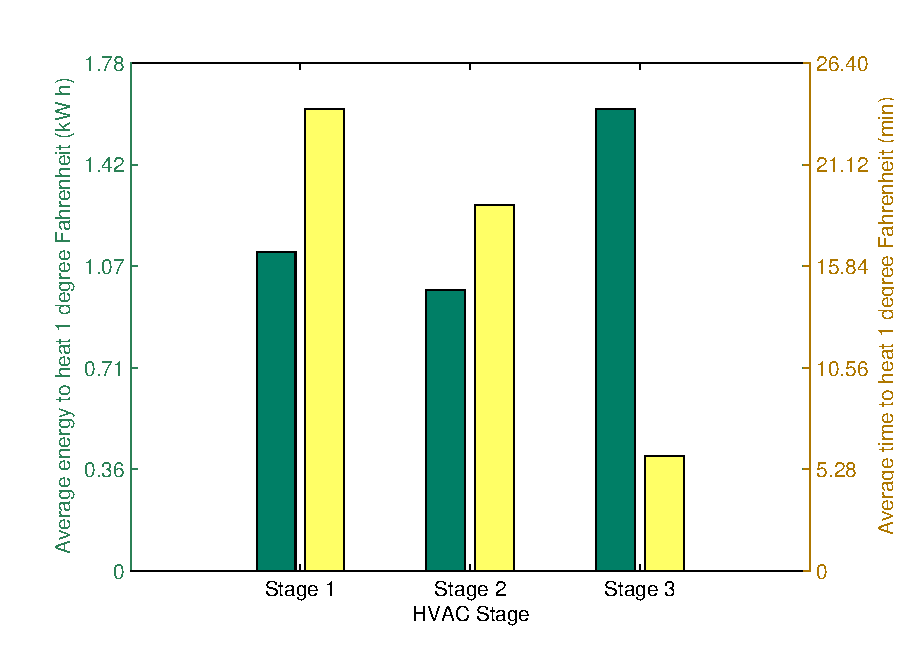
\includegraphics[width=0.6\columnwidth]{fig/stage_energy_lagtime}
\caption[Energy Efficiency and Lag Time for HVAC Heating Stages]{Energy
  efficiency and lag time vary among the multiple stages of HVAC.}
\label{fig:multistage}}
\end{figure}
% ----------------------------------------------------------------------------

The minimum airflow requirement makes selecting an efficient HVAC stage
challenging because there is a dependence between efficiency and airflow rate. As
Figure~\ref{fig:multistage} shows, stage 2 heating is the most energy efficient
stage for heating a room by one degree. Yet, as Table~\ref{table:stageAirflow}
shows, this stage produces conditioned air at a higher rate than stage 1
heating. Due to this, more rooms have to be open for stage 2 to be
usable. Therefore, a challenge for zone control is making this trade-off between
using efficient HVAC stages and minimizing the load on the selected stage so
that the rooms being conditioned reach the setpoint faster. 

\begin{table}[t]
{
  \begin{tabular}{|l|c|} \hline
    Stage & Air Output Rate (CFM) \\ \hline\hline
    Stage 1 Cool & 830
    \\ \hline
    Stage 2 Cool & 1200
    \\ \hline
    Stage 1 Heat & 775
    \\ \hline
    Stage 2 Heat & 1200
    \\ \hline
    Stage 3 Heat & 775
    \\ \hline
    \end{tabular}}
\caption[Conditioned Air Output for Different Heating and Cooling
  Stages]{Conditioned Air Output for Different Heating and Cooling Stages.}
\label{table:stageAirflow}
\end{table}

%% - thermal transfer

\subsection{Thermal Transfer}
\label{sec:thermalTransfer}
Thermal transfer between rooms has to be taken into consideration when deciding
on rooms to be conditioned at any given time. For instance, in a house with an
open floor-plan with the kitchen and living room sharing a large opening between
them, attempting to condition the living room and not the kitchen, or vice
versa, would cause a wastage in energy due to the large amount of leakage of
conditioned air from the conditioned room to the unconditioned room. In such a
situation maintaining dependent rooms at a temperature close to the rooms being
conditioned would reduce the energy wastage by decreasing the temperature
gradient between the rooms. Thus, identifying these inter-dependencies is a
challenge that has to be addressed for zone control.

\section{Approach}
%% - Minimize system state changes 
%%  - Maximize stability

Our approach to zone control involves attempting to maximize the stability of
the system by minimizing the number of system changes. Thus, at any decision
point Smart Zoning attempts to maintain the damper and HVAC equipment at their
current state unless changing their state would greatly decrease the estimated
energy used, or leaving the system at its current state would considerably
affect resident comfort.

%------------------------------------------------------------------------------
% Figure 5
\begin{figure}[t]
\centering{
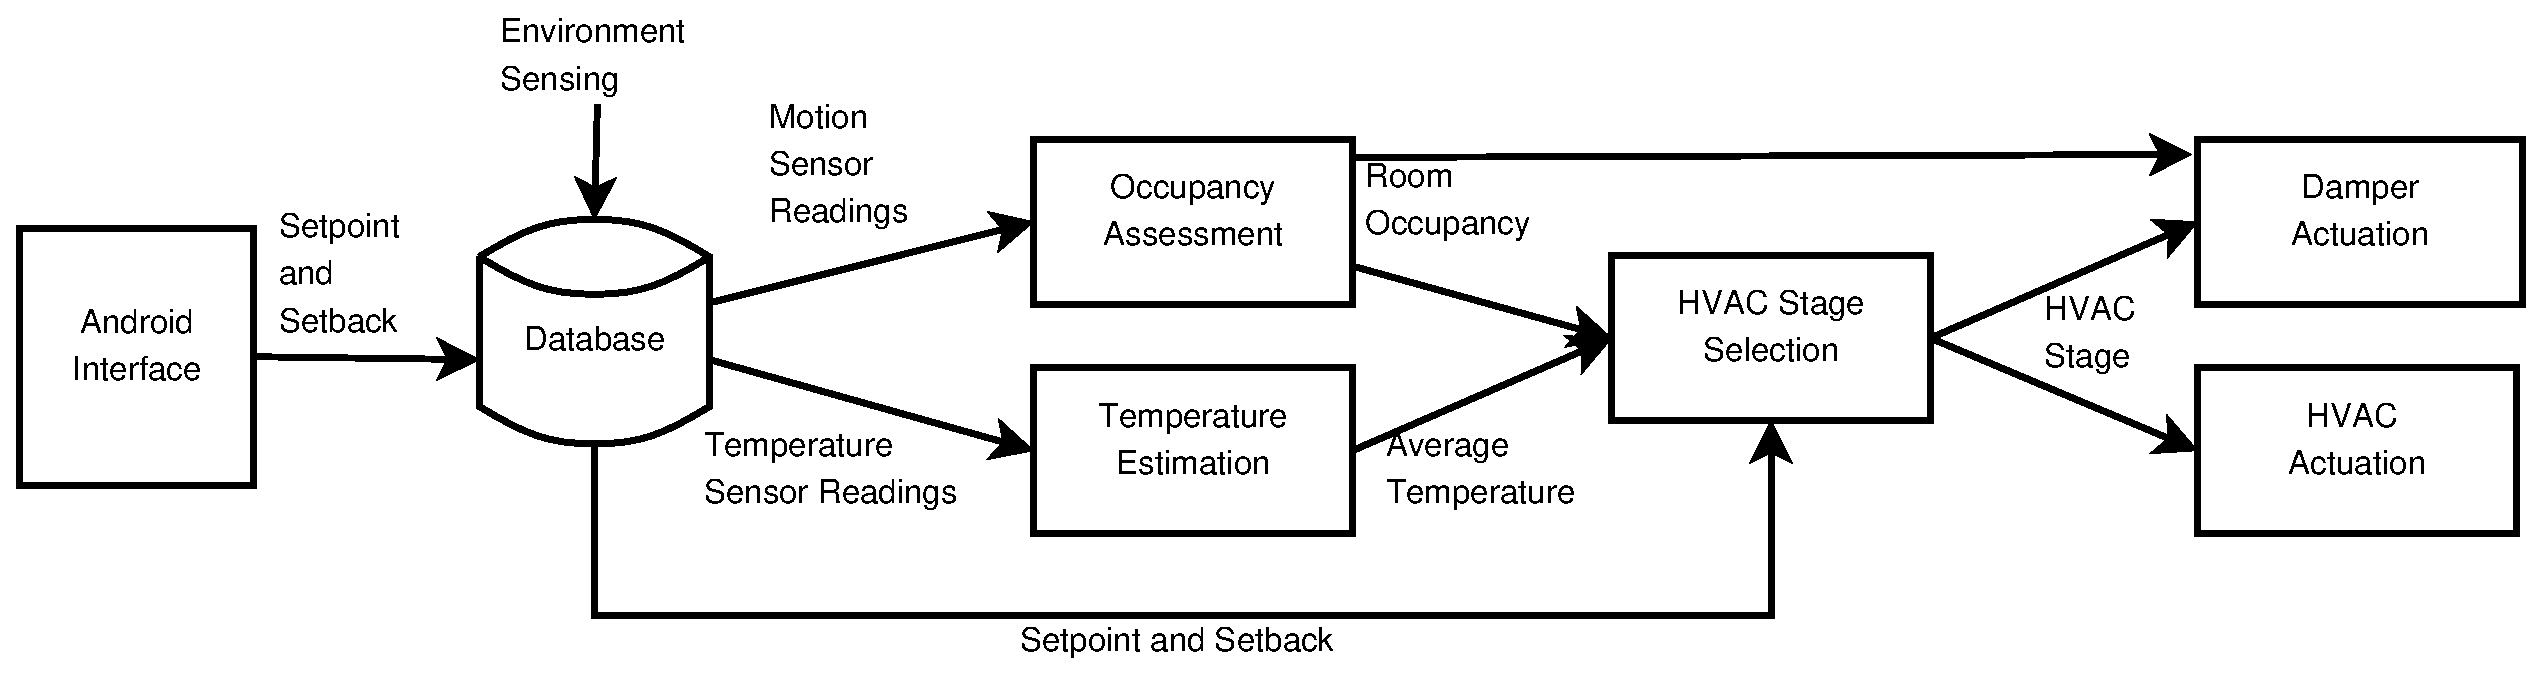
\includegraphics[width=0.9\columnwidth]{fig/controlFlow}
\caption[Zone Control Data Flow Diagram]{The data flow through the zone control algorithm.}
\label{fig:zoneControl}}
\end{figure}
% ----------------------------------------------------------------------------

Figure~\ref{fig:zoneControl} shows the main modules that encompass the zone
controller and the flow of data through the system. All sensor readings, from
temperature and occupancy sensors, are written to a database in real-time. The
database also holds the setpoint and setback temperature as input by the
resident through an Android smartphone-based user interface. These values are
read from the database by the zone controller and used to assess occupancy, as
described in Section~\ref{sec:occupancyAssessment} and estimate an average
temperature as will be described in Section~\ref{sec:temperatureEstimation}. The
room occupancy results and average temperature are used to decide upon the HVAC
stage to be used when actuating the HVAC equipment. The HVAC stage decide upon,
along with the room occupancy assessment results, are used to decide on the
dampers to actuate.

\subsection{Temperature Estimation}
\label{sec:temperatureEstimation}
Room-level zoning would seem to indicate that the desired mode for temperature
sensing would be at the room level. Yet, reacting to room-level temperature
fluctuations requires many, frequent, system changes decreasing the stability of
the system. This could be caused by the movement of residents through the house
causing the set of occupied rooms to change. If any of the newly occupied rooms
has a temperature significantly different from other rooms, due to not being
occupied for a while for instance, this single room could dramatically affect
the system state. Relying on room-level temperatures could also cause the system
to be extremely sensitive to environmental variations in the house.  For
instance, a South-facing room would be influenced by sunlight much more than a
room facing any other direction and if such a room becomes occupied, its
temperature would greatly skew the zone controller. Due to these issues, our
approach for obtaining a temperature to be used to make control decisions
involves calculating an average temperature as described in
Algorithm~\ref{alg:temperatureEstimation}. 

\begin{algorithm}                      % enter the algorithm environment
\caption{Temperature Estimation}          % give the algorithm a caption
\label{alg:temperatureEstimation}% and a label for \ref{} commands later in the document
\begin{algorithmic}                    % enter the algorithmic environment
\STATE $wholeHouseTempSum = 0$
\STATE $numRooms = 0$
\FOR{$room in rooms$}
\STATE $wholeHouseTempSum += room.temperature$
\STATE $numRooms += 1$
\ENDFOR
\STATE $wholeHouseAvg = wholeHouseTempSum / numRooms$

\STATE $conditionedRoomsTempSum = 0$
\STATE $numConditionedRooms = 0$
\FOR{$room in rooms$}
\IF{$room.damperClosed == False \: \AND \: room.transitionallyOccupied ==
  False$}
\STATE $conditionedRoomsTempSum += room.temperature$
\STATE $numConditionedRooms += 1$
\ENDIF
\ENDFOR
\STATE $conditionedRoomsAvg = conditionedRoomsTempSum / numConditionedRooms$

\STATE $occupiedRoomsTempSum = 0$
\STATE $numOccupiedRooms = 0$
\FOR{$room in rooms$}
\IF{$room.stablyOccupied$}
\STATE $occupiedRoomsTempSum += room.temperature$
\STATE $numOccupiedRooms += 1$
\ENDIF
\ENDFOR
\STATE $occupiedRoomsAvg = occupiedRoomsTempSum / numOccupiedRooms$
\IF{$mode == 'cool'$}
\STATE $averageTemp = min(wholeHouseAvg, conditionedRoomsAvg,
occupiedRoomsAvg)$
\ELSE
\STATE $averageTemp = max(wholeHouseAvg, conditionedRoomsAvg,
occupiedRoomsAvg)$
\ENDIF
\end{algorithmic}
\end{algorithm}

The temperature estimation algorithm (Algorithm~\ref{alg:temperatureEstimation})
calculates three separate average temperatures: (i) the average temperature
across the whole house, (ii) the average temperature of rooms that are being
conditioned, and (iii) the average temperature of rooms that are occupied. The
difference between the second and third average temperatures is that rooms that
are unoccupied can also be conditioned, with their dampers open letting
conditioned air in, due to them being selected as dump zones as will be
described in Section~\ref{sec:damperActuation}. When the HVAC system is being
used to cool the house, in the summer for instance, the minimum of these
temperatures is used as the average temperature for zone control. When the HVAC
system is used for heating, the maximum of these three values is used.

\subsection{HVAC Stage Selection}
\label{sec:hvacStageSelection}

The HVAC stage selection algorithm uses the assessed room occupancies, average
temperature, setpoint, and setback to select the stage with which the HVAC
equipment should be actuated using hysteresis to prevent wild swings between
HVAC stages.

\begin{algorithm}                      % enter the algorithm environment
\caption{HVAC Stage Selection}          % give the algorithm a caption
\label{alg:hvacStageSelection}% and a label for \ref{} commands later in the document
\begin{algorithmic}                    % enter the algorithmic environment
\IF{$numOccupiedRooms > 0$}
\STATE $tempDiff = averageTemp - setpoint$
\ELSE
\STATE $tempDiff = averageTemp - setback$
\ENDIF

\IF{$mode == 'heat'$}
\STATE $tempDiff = -tempDiff$
\ENDIF

\IF{$hvacStage == -1$}
\IF{$tempDiff > 1.5$}
\STATE $hvacStage = 2$
\ELSIF{$tempDiff > 0.5$}
\STATE $hvacStage = 1$
\ELSE
\STATE $hvacStage = 0$
\ENDIF
\ELSIF{$hvacStage == 0$}
\IF{$tempDiff > 1.7$}
\STATE $hvacStage = 2$
\ELSIF{$tempDiff > 0.7$}
\STATE $hvacStage = 1$
\ENDIF
\ELSIF{$hvacStage == 1$}
\IF{$tempDiff > 1.7$}
\STATE $hvacStage = 2$
\ELSIF{$tempDiff < -0.5$}
\STATE $hvacStage = 0$
\ENDIF
\ELSE
\IF{$tempDiff < -0.5$}
\STATE $hvacStage = 0$
\ELSIF{$tempDiff < 0.3$}
\STATE $hvacStage = 1$
\ENDIF
\ENDIF
\end{algorithmic}
\end{algorithm}

Algorithm~\ref{alg:hvacStageSelection} describes the algorithm used for
selecting the HVAC stage. If any room in the house is occupied, the difference
between the setpoint, a comfortable temperature set by the resident, and the
average temperature, as calculated using
Algorithm~\ref{alg:temperatureEstimation}, is used to select the HVAC stage. If
the house is unoccupied, the difference is calculated between the setback
temperature, an energy saving temperature that is warmer than the setpoint in
summer and colder than the setpoint in winter, and the average temperature. A
finite-state machine (Figure~\ref{fig:fsm}), with four states, is used to decide
on the HVAC stage. The initialization state is defined as $-1$, and $0$
indicates the HVAC system being turned off. States $1$ and $2$ correspond to the
HVAC stages described in Section~\ref{sec:efficiencyDependence}.

%------------------------------------------------------------------------------
% Figure 5
\begin{figure}[t]
\centering{
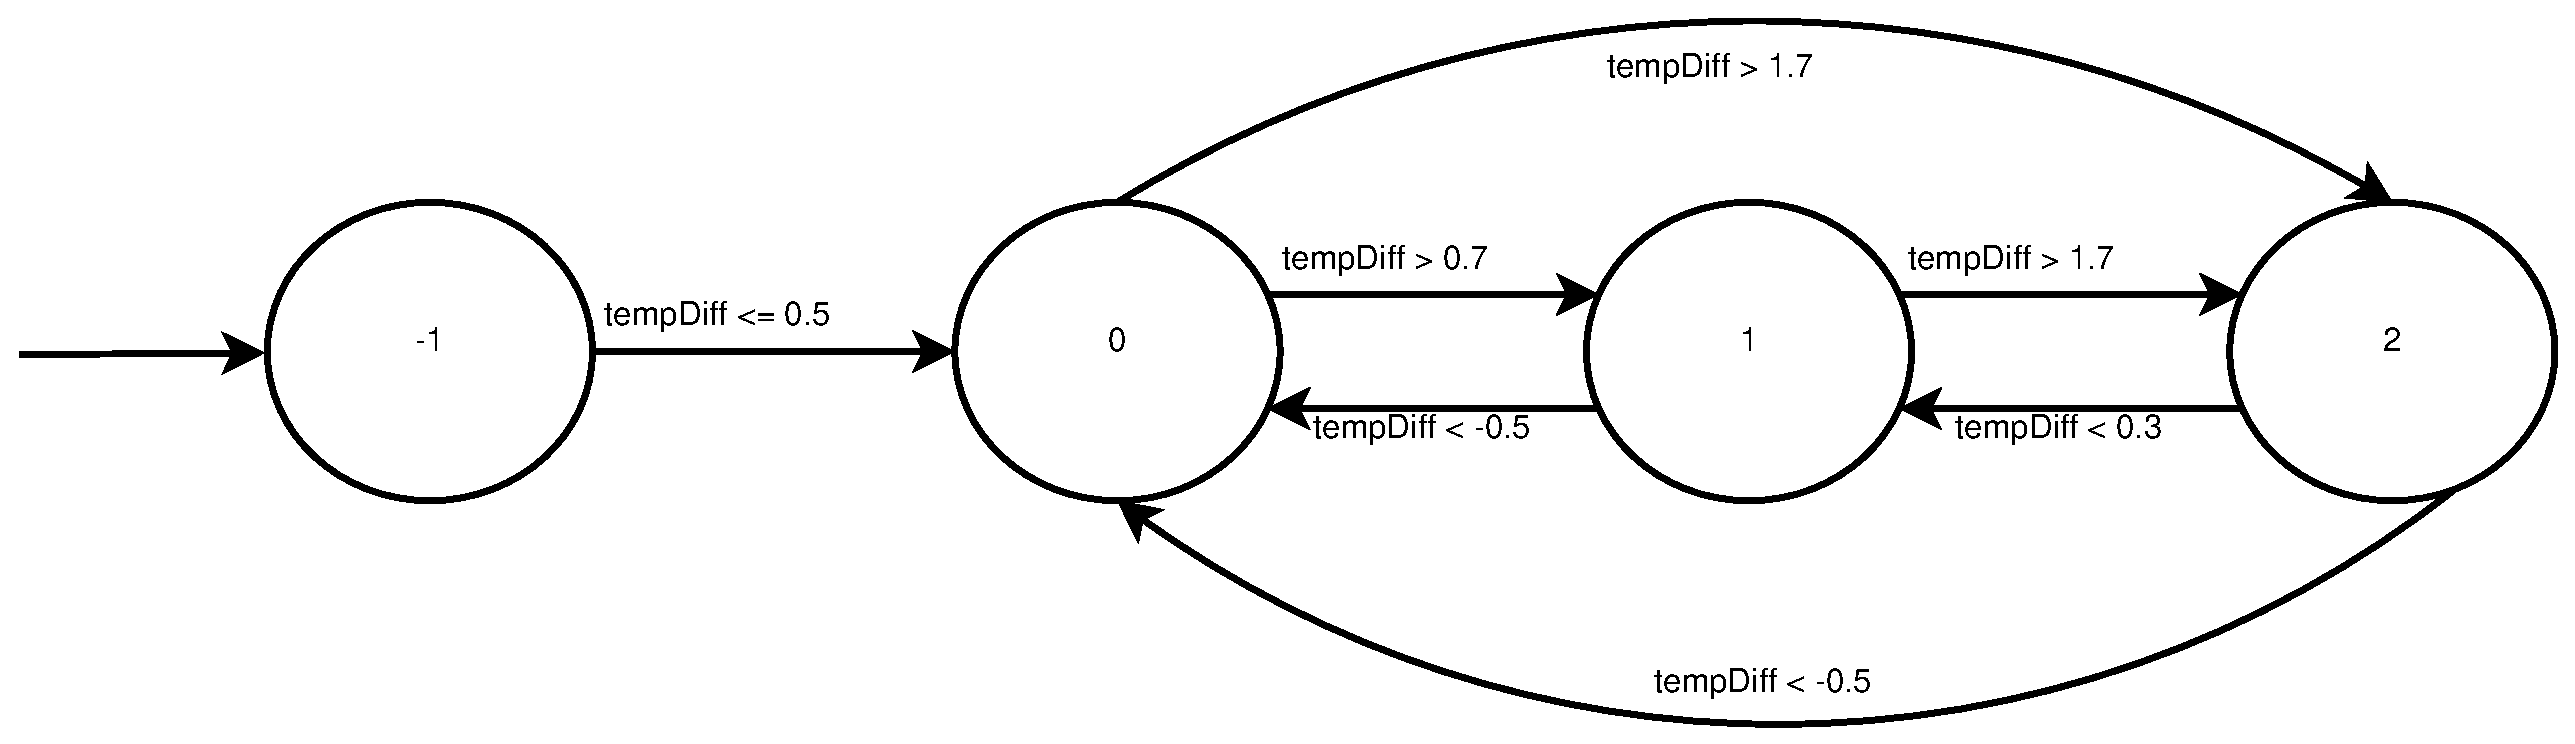
\includegraphics[width=0.9\columnwidth]{fig/stateMachine}
\caption[Finite-State Machine Used for HVAC Stage Selection.]{The finite-state
  machine which provides hysteresis during the stage selection process..}
\label{fig:fsm}}
\end{figure}
% ----------------------------------------------------------------------------

\subsection{Damper Actuation}
\label{sec:damperActuation}

%% - Open all ``occ''
%%  -> no room-level temperature control

Damper actuation involves selecting the dampers to be opened and closed and
sending the appropriate commands to the damper control circuitry. Since the zone
controller does not use room-level temperature control, as described in
Section~\ref{sec:temperatureEstimation}, all rooms that are occupied have their
dampers open. The decision that has to be made is on what additional rooms,
called {\em dump rooms}, that comprise the {\em dump zone} have to be opened, if
they are closed. This decision is based on ensuring the safety of the HVAC
equipment by minimizing the chance of back-pressure buildup due to too many
dampers being closed. As described in
Section~\ref{sec:efficiencyDependence}, the HVAC stage selected by
Algorithm~\ref{alg:hvacStageSelection} determines the minimum airflow into the
rooms in order to ensure equipment safety. Thus, the damper actuation module
attempts to ensure this minimum airflow by strategically opening additional
rooms as needed so that there is minimum impact to the efficiency with which the
occupied rooms are conditioned. 

\begin{algorithm}                      % enter the algorithm environment
\caption{Dump Zone Selection}          % give the algorithm a caption
\label{alg:dumpZoneSelection}% and a label for \ref{} commands later in the document
\begin{algorithmic}                    % enter the algorithmic environment
\FOR{$room in rooms$}
\STATE $activeRooms = []$
\STATE $dumpCandidate = []$
\IF{$room.stageRequest > 0 or room.transitionallyOccupied$}
\STATE $activeRooms.append(room)$
\ELSE
\STATE $dumpCandidates.append(room)$
\ENDIF
\ENDFOR

\STATE $dumpSets = []$

\FOR{$dumpSet in combinations(dumpCandidates)$}

\STATE $airflow = calculateAirflow(activeRooms, dumpSet)$

\STATE $minFlowChange = INF$
\FOR{$room in dumpSet$}
\IF{$room.openAirflow < minflow$}
\STATE $minFlowChange = room.openAirflow - room.closedAirflow$
\ENDIF
\ENDFOR

\IF{$airflow > safeAirflow \: \AND \: minFlowChange > airflow - safeAirflow$}
\STATE $dumpSets.append(dumpSet)$
\ENDIF

\ENDFOR

\STATE $bestEnergy = -INF$
\STATE $bestDamperChanges = 0$
\STATE $bestDumpZone = []$
\FOR{$dumpSet in dumpSets$}

\STATE $inactiveRooms = rooms$
\FOR{$room in activeRooms$}
\STATE $inactiveRooms.remove(room)$
\STATE $activeZoneEnergy += voltages(hvacStage, dumpSet, room)$
\ENDFOR

\STATE $damperChanges = 0$
\FOR{$room in dumpSet$}
\STATE $inactiveRooms.remove(room)$
\IF{$room.damperClosed$}
\STATE $damperChanges += 1$
\ENDIF
\ENDFOR

\FOR{$room in inactiveRooms$}
\IF{$room.damperClosed == False$}
\STATE $damperChanges += 1$
\ENDIF
\ENDFOR

\IF{$activeZoneEnergy - damperPenalty * damperChanges > bestEnergy -
  damperPenalty * bestDamperChanges$}
\STATE $bestDumpZone = dumpSet$
\STATE $bestEnergy = activeZoneEnergy$
\STATE $bestDamperChanges = damperChanges$
\ENDIF

\ENDFOR

\STATE $dumpZone = []$
\FOR{$room in bestDumpZone$}
\STATE $dumpZone.append(room)$
\STATE $estimatedAirflow = calculateAirflow(activeRooms, dumpZone)$
\IF{$estimatedAirflow > safeAirflow$}
\STATE $return dumpZone$
\ENDIF
\ENDFOR

\end{algorithmic}
\end{algorithm}

%% - dump when needed
%%  - dump zones based on thermal transfer
%%    - not temp

%% - keep old occupied rooms as dump zones

Algorithm~\ref{alg:dumpZoneSelection} is used during zone control to select the
rooms that comprise the dump zone. Whenever there are insufficient rooms
occupied in order to ensure sufficient airflow out of the ducts, the dump zone
selection algorithm is called. This algorithm selects dump zones based on the
estimated benefit, in terms of thermal transfer, to the occupied rooms rather
than the actual temperatures of the potential dump rooms. Also, the algorithm
prefers rooms that have been occupied in the near past as dump rooms. These
approaches to dump zone selection ensures the zone controller is able to achieve
its goal of maximizing system stability by minimizing state changes.

The first phase of dump zone selection is separating the rooms into active
rooms, those room that require conditioning due to either being stably, or
transitionally, occupied or being beyond the setback temperature, and dump
candidates. Next, all combinations of dump candidates are evaluated in order to
identify the set of rooms that have the greatest positive impact on the goals of
zone control. 

The first step in dump candidate evaluation is estimating the total airflow out
of the ducts with a particular set of dump rooms. We use the airflow calculation
technique described in Algorithm~\ref{alg:calculateAirflow} in order to achieve
this. This algorithm uses empirical values of airflow, measured using a airflow
meter, in order to estimate the airflow. We use a conservative approach to
airflow estimation by using measurements from a single register being closed at
a time. Thus, we use empirical values from each register being open, when all
other registers are open, as their {\em openAirflows} and each register being
closed, when all other registers are open, as their {\em closedAirflow}. This
approach gives us a lower bound on airflow since closing any other register
concurrently with the one being measured would increase the airflow from the
measured register. We take this approach to minimize the number of measurements
that have to be taken since for a house with 13 registers, as the house we
evaluated the system on contained, it would take $2^{13} = 8192$ measurements in
order to have airflow values for all combinations of register openings and
closings which would be more than two weeks of manual data collection. Our
approach enabled all the data to be collected within a few hours.

\begin{algorithm}                      % enter the algorithm environment
\caption{Airflow Calculation}          % give the algorithm a caption
\label{alg:calculateAirflow}% and a label for \ref{} commands later in the document
\begin{algorithmic}                    % enter the algorithmic environment
\STATE $airflow = 0$
\FOR{$room in rooms$}
\IF{$room in activeRooms \: \OR \: dumpSet$}
\STATE $airflow += room.openAirflow$
\ELSE
\STATE $airflow += room.closedAirflow$
\ENDIF
\ENDFOR
\end{algorithmic}
\end{algorithm}

The estimated airflow is used to eliminate dump candidates that would not help
with ensuring a safe volume of airflow out of the system. In addition to
ensuring that this safety limit is met, we also verify that no room in the set
can be removed and still have a safe airflow out of the system using the minimum
airflow change which is the minimum difference in airflow from a room in the set
being opened and closed. This minimum airflow change is compared to the
difference between the airflow estimate and the safe airflow to ensure that the
change is greater than the difference and therefore the room has to be opened. 

%% The next step of dump zone selection is optimizing over the search space of dump
%% candidates that passed the airflow check. The optimization is done over two
%% parameters: {\em zone energy} and {\em damper changes}. Zone energy is an
%% estimate of the thermal impact on occupied rooms by a particular dump zone and
%% damper changes is the number of rooms that have to be changed from currently
%% being opened to closed, or closed to opened. Zone energy is calculated using
%% voltage values that are obtained from a circuit model of airflow in a house that
%% we define as described in Section~\ref{sec:circuitModel}. This model assume
%% rooms are wires with resistors between them and the air coming out of the
%% dampers are current sources. Give a set of current sources, as estimated
%% airflows from the registers, the model provides voltages for each room. These
%% voltages describe temperature changes in rooms with higher voltages indicating a
%% greater temperature change. Thus, the optimization function attempts to search
%% for dump zones that have the greatest impact on the voltage of the occupied
%% rooms, indicating the possibility of the greatest positive impact on those rooms
%% in terms of thermal transfer. With this approach we address the thermal transfer
%% challenge as described in Section~\ref{sec:thermalTransfer}. In addition to the
%% zone energy, we also attempt to minimize the number of damper changes that have
%% to be made to achieve the dump zone. This ensures that rooms that were recently
%% occupied are preferred as dump candidates since their dampers are more likely to
%% be open and also minimizes the number of state changes necessary, as the zoning
%% controller is trying to achieve. Preferring recently occupied rooms helps ensure
%% that rooms that are used in mult-room occupancy scenarios are kept close to the
%% setpoint. This also helps ensure that the temperature of rooms that are more
%% likely to be occupied in the future, due to temporal locality, are not allowed
%% to drift far from the setpoint.

%% \section{Evaluation}
